
\chapter{Introduction\label{ch:intro}}

Our understanding of fundamental particles and interactions has progressed much from the early days.
These beginnings could be with Empdocles and his four roots fire, earth, air, and water, or with
Aristotle relating these four roots to two of the four sensible quantities hot, dry, wet, and
cold~\cite{0415078547} as in Figure~\ref{fig:aristotle}
(not to omit classical elements from other philosophies and worldviews), or more recently with
John Dalton's atoms~\cite{dalton}. Or perhaps particle physics began with
the discovery of the electron by J.J. Thomson in 1897~\cite{thomson:electron},
which to this day has not been observed
to have internal structure or decay, with upper (lower) bounds on the radius (lifetime) of
10$^{-22}$~m (10$^{26}$~years)~\cite{1988PhST...22..102D,2002PhLB..525...29B}.

\begin{figure}[ht]
 \begin{center}
    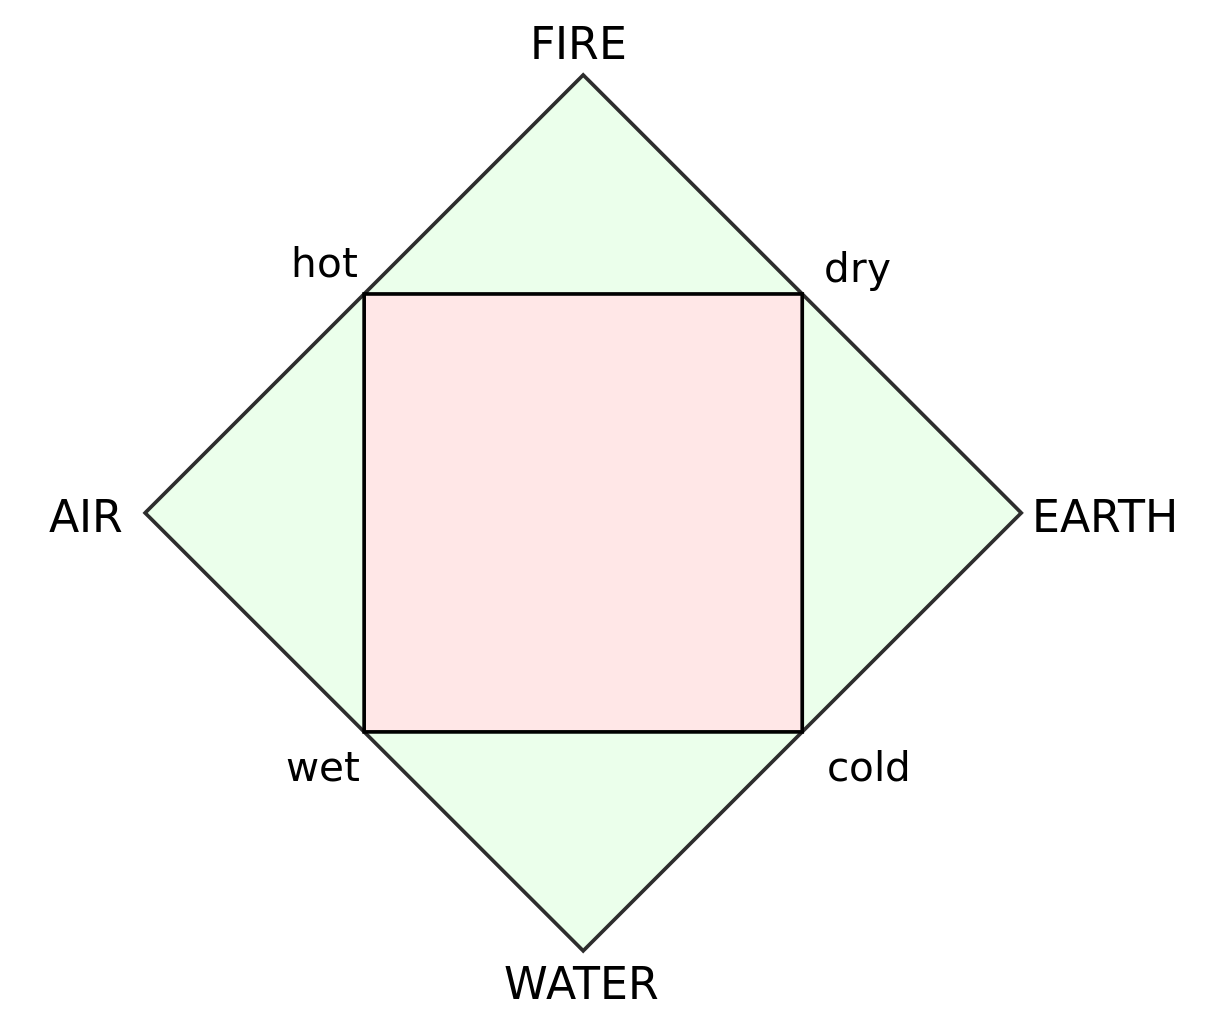
\includegraphics[width=0.90\textwidth]{figures/intro/Four_elements_representation.png}
      \end{center}
\caption{The four roots how they relate to the sensible quantities.}
\label{fig:aristotle}
\end{figure}

Today we have the Standard Model, the theoretical framework that best describes the
experimentally oberserved phenomena of the fundamental particles and their interactions. The theory
is not perfect, and it remains an overarching theme of particle physics to unify physical processes
at all energy scales under one single framework, if such a thing can be done at all.
The SM and its shortcomings are described in
Sections~\ref{sec:SM} and \ref{sec:SMshortcomings}.

Recently in 2012, the last piece to the SM was put into place with the discovery of the Higgs boson.
This discovery, described in Section~\ref{sec:discovery}, is the foundation for the work based on
this thesis, the goal of which is to describe the first search for diHiggs production, a process
in which two Higgs bosons are produced. The motivations for what the search for this process means
in the context of SM physics and ``new'' physics is given in Section~\ref{sec:diHiggs}.

Finally, for those readers who have by chance come across this thesis and do not
have any physics training, Appendix~\ref{ch:mom} may be especially appealing.

\section{The Standard Model\label{sec:SM}}

The Standard Model (SM) of particle physics is a relativistic quantum field theory
that describes how the known fundamental particles interact through the electromagnetic, weak,
and strong forces.
The theory was developed through the unification of the electromagnetic and weak forces by Glashow
in 1961~\cite{1961.Glashow.Partial-symmetries} and through the incorporation of this electroweak
theory with the Higgs mechanism by Weinberg and Salam in 1967~\cite{PhysRevLett.19.1264,Salam:1968rm}.
This theory explained the experimental observations of the day, and later experiments provided
additional evidence as well as a mean for measuring the free parameters of the theory. Some of
this evidence is provided in Figure~\ref{fig:discoveries} in the form of the discoveries of
the fundamental particles.

\begin{figure}[ht]
 \begin{center}
    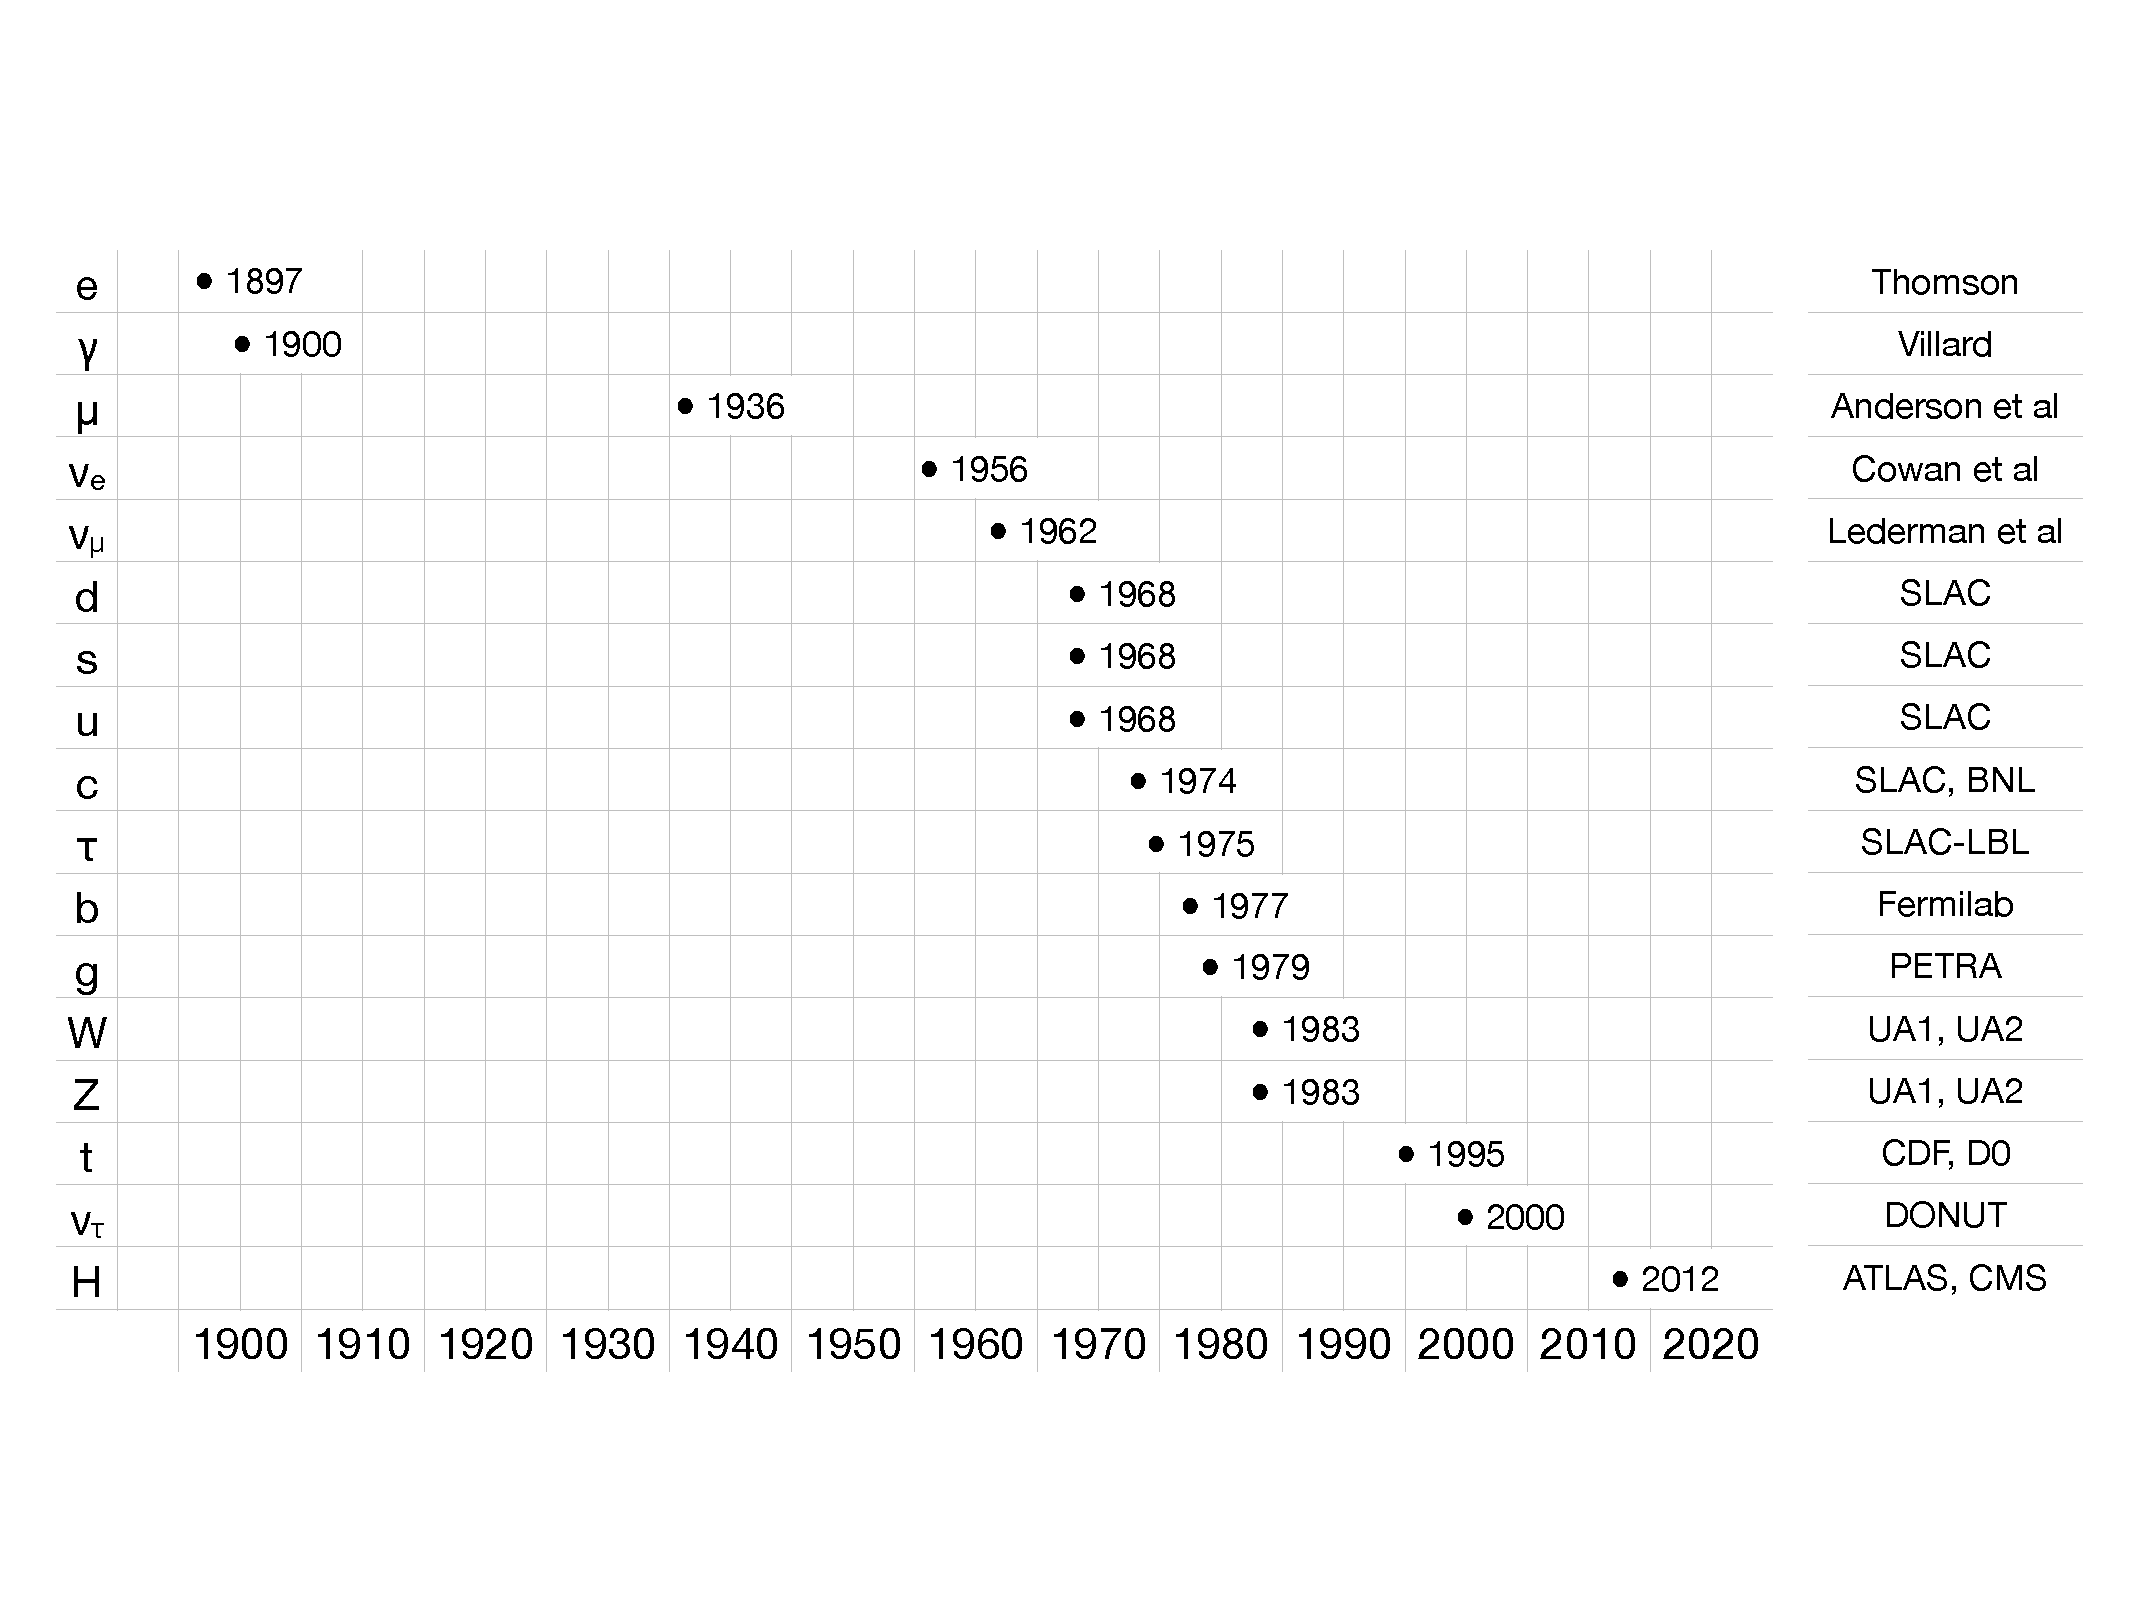
\includegraphics[width=0.90\textwidth]{figures/intro/discoveries.pdf}
      \end{center}
\caption{The discoveries of fundamental particles versus time~\cite{Tuna:thesis}.}
\label{fig:discoveries}
\end{figure}

In this theory, particles are treated as excitations of fields having half-integer spin or
integer spin, and the forces are treated as interactions among excitations of these fields.
The spin-$\frac{1}{2}$ particles, or fermions, can be divided into groups based on the ways
in which they interact. The leptons, or those particles which only experience the electroweak force,
are the electron $e$, muon $\mu$, tau $\tau$, electron neutrino $\nu_e$, muon neutrino $\nu_\mu$, and
tau neutrino $\nu_\tau$. The quarks, or those particles which experience both electoweak and strong
forces, are the up $u$, down $d$, strange $s$, charm $c$, bottom $b$, and top $t$. The integer-spin
particles, or bosons, are the spin-1 photon $\gamma$, $W$, $Z$, and gluon $g$ and the spin-0 Higgs $H$.
The particle content of the SM is summarized in Figure~\ref{fig:SMtable}.

\begin{figure}[ht]
 \begin{center}
    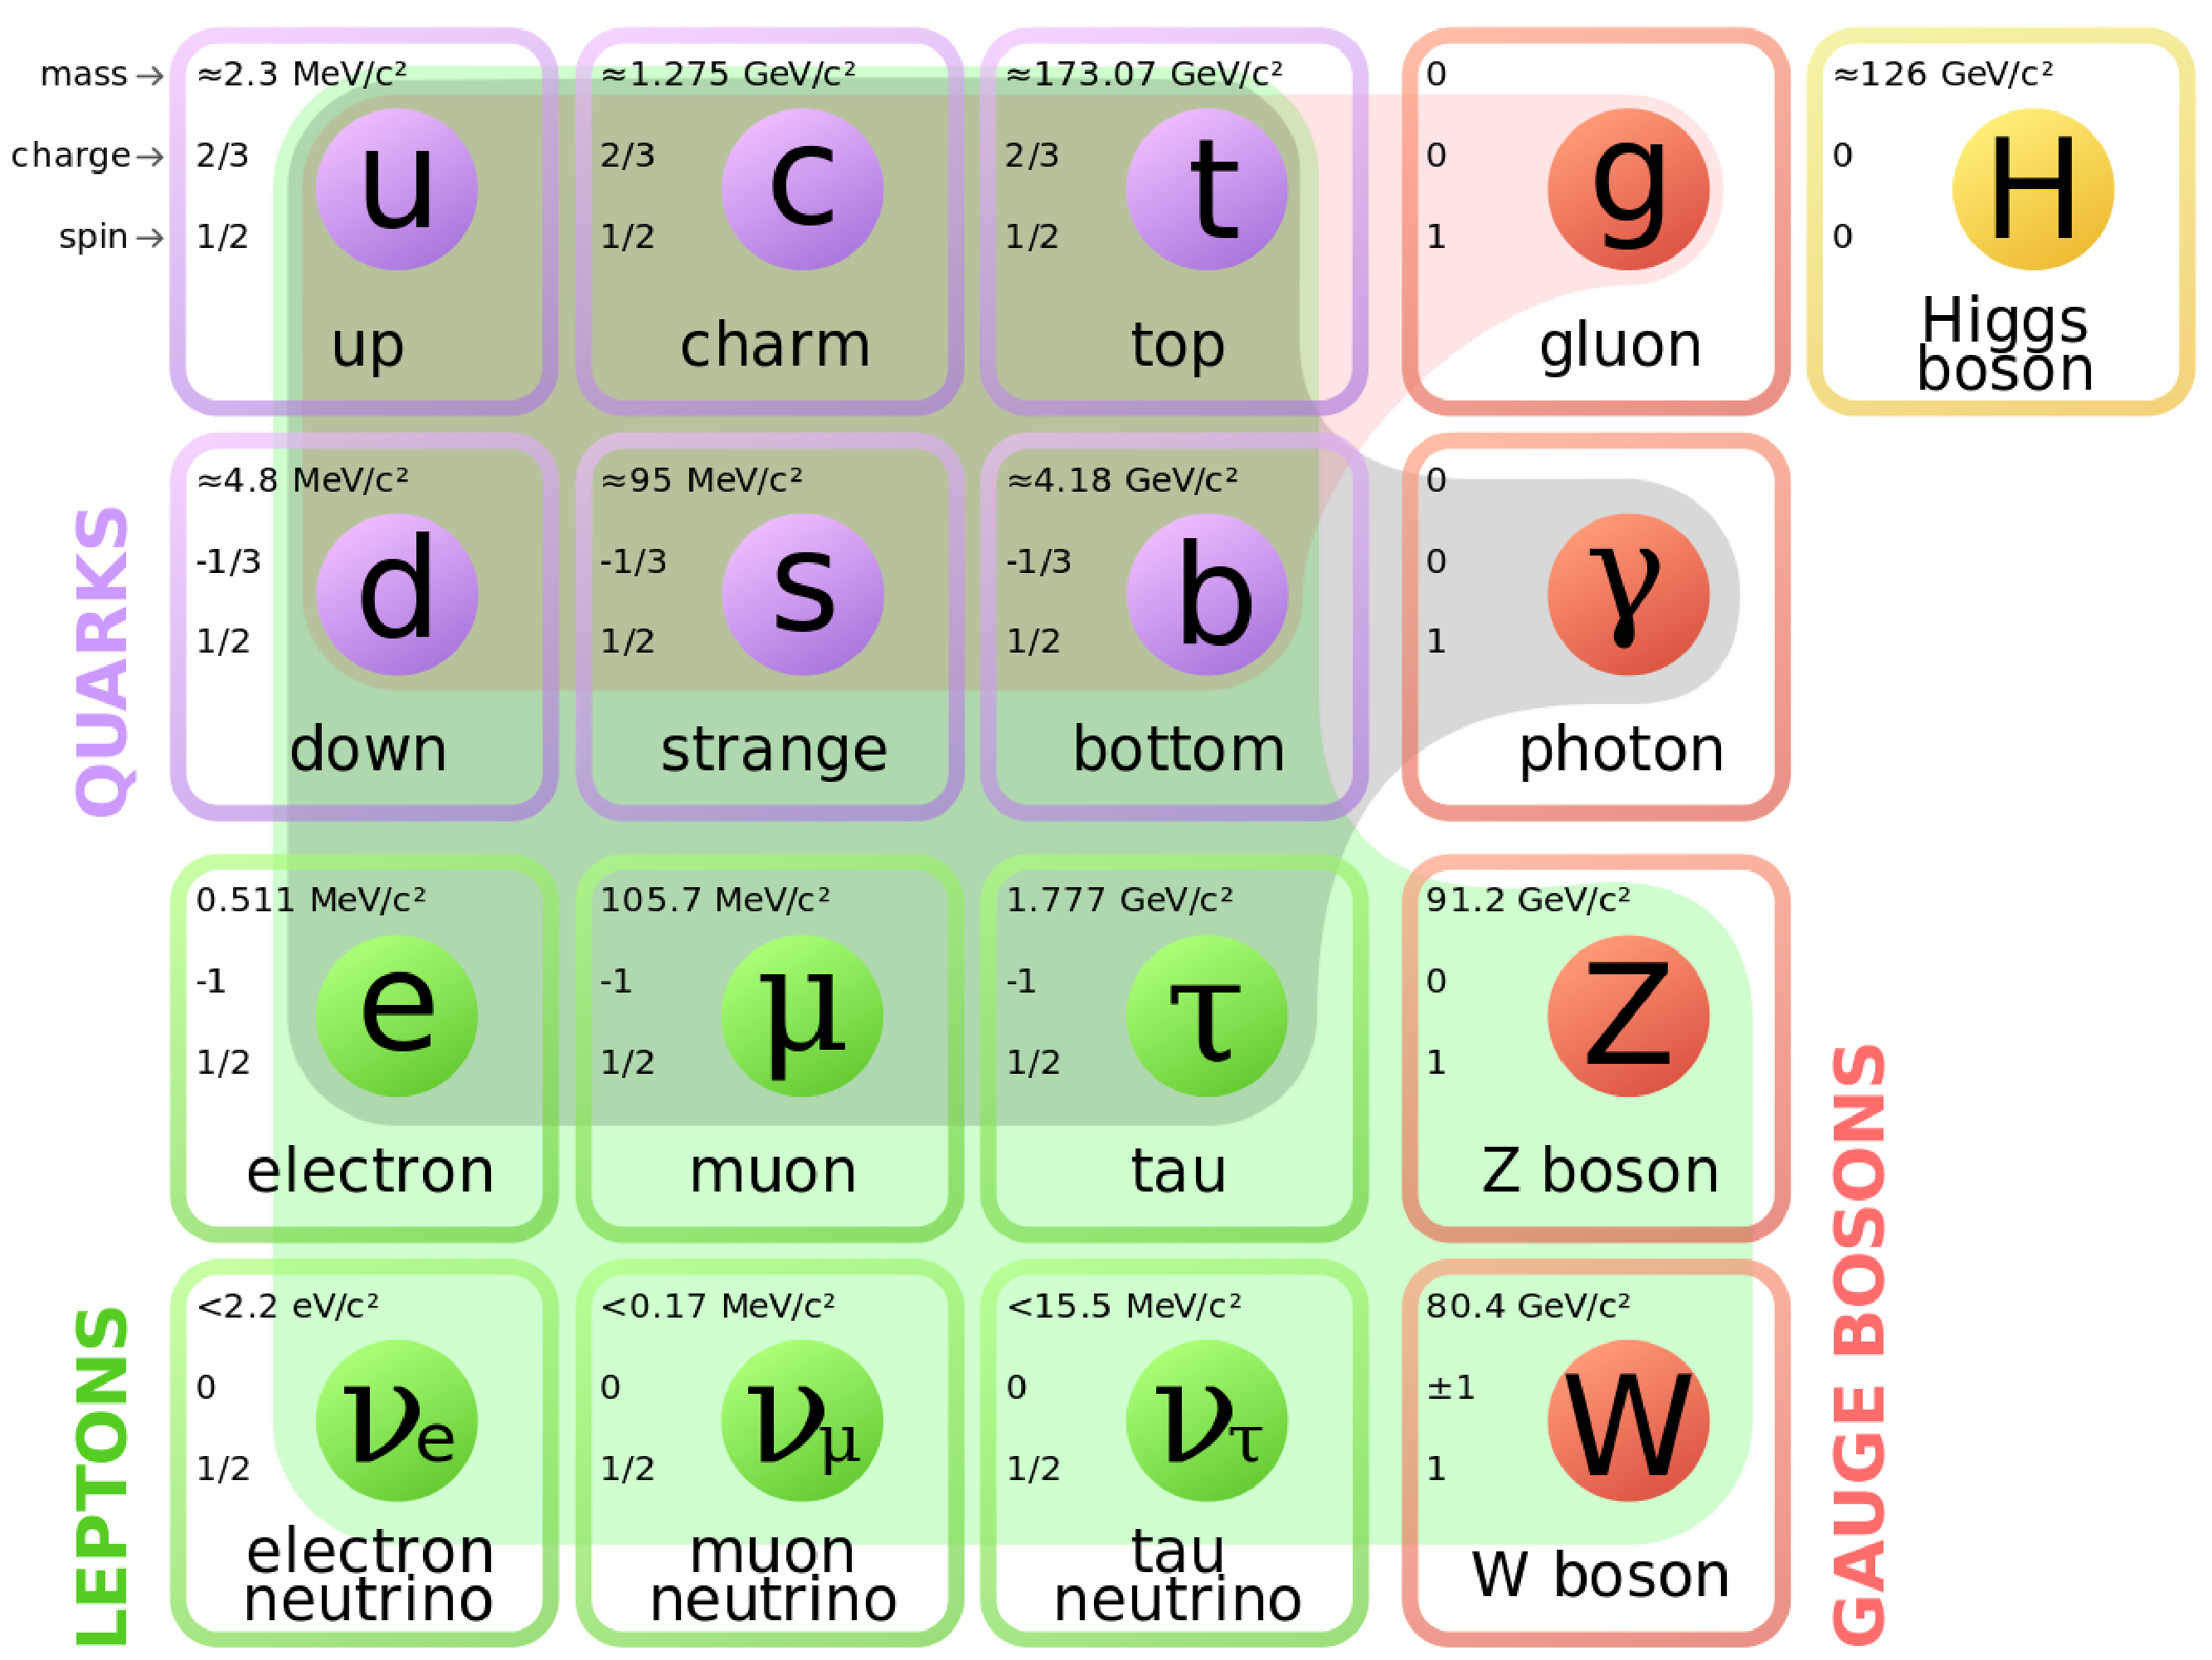
\includegraphics[width=0.90\textwidth]{figures/intro/Standard_Model_of_Elementary_Particles_modified_version.pdf}
      \end{center}
\caption{A diagram of the particle content of the SM~\cite{SMdiagram}.
The mass, electric charge, and spin is given for each, and the background color indicates how each
fermion interacts with the bosons.}
\label{fig:SMtable}
\end{figure}

The dynamics of the SM are described through its Lagrangian, which is invariant under
gauge transformations of the group ${\rm SU(3)}_C \times {\rm SU(2)}_L \times {\rm U(1)}_Y$.
The strong force is associated with transformations under ${\rm SU(3)}_C$, which give rise to
the conserved color charge $C$, denoted red, green, or blue, and eight gauge fields.
The group acts on 18 spinor fields corresponding to the quarks (six quark flavors in three colors)
and the eight gauge fields corresponding to the gluons.
The electroweak force is associated with transformations under ${\rm SU(2)}_L \times {\rm U(1)}_Y$,
the first part of which give rise to the conserved left-handed chirality $L$ and three gauge fields,
and the second part of which gives rise to the conserved weak hypercharge $Y$ one gauge field.
This group acts on left-handed doublets and right-handed singlets of the quarks, leptons, and
these four gauge fields. The quarks contribute nine doublets and 18 singlets, and the leptons contribute
three doublets and three singlets (as right-handed neutrinos do not exist).

The symmetry group of the SM does not allow for gauge-invariant mass terms. Instead,
the generation of particle masses is accomplished through the partial breaking of the
symmetry group by the addition of the Higgs field and potential, after which gauge-invariant
Yukawa interactions between fermions and the Higgs field naturally give fermion masses.
The Higgs field $\phi$ is a doublet of ${\rm SU(2)}_L$, and its potential takes the form
\begin{equation}
V(\phi^\dagger\phi) = -\mu\phi^\dagger\phi + \lambda(\phi^\dagger\phi)^2 \,,
\end{equation}
where $\mu,\lambda > 0$. The ground state of this potential is nonzero and degenerate. With the
choose of a convient gauge, the ground state can be expressed as
\begin{equation}
\left\langle \phi \right\rangle =
\left\langle \frac{1}{\sqrt{2}} {\phi^0+i\phi^1 \choose \phi^2+i\phi^3} \right\rangle =
{\mu / \sqrt{\lambda} \choose 0} \,,
\end{equation}
where $\phi^1, \phi^2, \phi^3$ are massless Goldstone
bosons~\cite{1961.Goldstone,1962.Goldstone-Salam-Weinberg.Broken-Symmetries} and the remaining
degree of freedom represents fluctuations about this ground state,
associated with the massive scalar Higgs boson $H$.

Recalling that the Higgs field is a doublet of ${\rm SU(2)}_L$, its covariant derivative in the
Langrangian is
\begin{equation}
D_\mu = \partial_\mu - i g_1 T^a W^a_\mu - i \frac{g_2}{2} B_\mu \,,
\end{equation}
where $g_1$ ($g_2$) and $W^a_\mu$ ($B_\mu$) are the gauge couplings and three (one) gauge bosons
associated with ${\rm SU(2)}_L$ (${\rm U(1)}_Y$), respectively, and $T^a$ are the generators of
${\rm SU(2)}_L$. The ground state of the Higgs field then gives mass terms to some of the gauge bosons.
The mass eigenstates, in terms of the $W^a_\mu$ and $B_\mu$, are the $W^\pm$, $Z$, and photon with
masses
\begin{subequations}
\begin{equation}
m_{W^\pm} = \frac{g_1}{2}\frac{\mu}{\sqrt{\lambda}}
\end{equation}
\begin{equation}
m_Z = \frac{\sqrt{g_1^2+g_2^2}}{2}\frac{\mu}{\sqrt{\lambda}}
\end{equation}
\begin{equation}
m_\gamma = 0 \,.
\end{equation}
\end{subequations}
Thus, the gauge bosons acquire mass, and the symmetry of ${\rm SU(2)}_L \times {\rm U(1)}_Y$ is
broken to ${\rm U(1)}_{EM}$ with gauge field being the photon.  

Masses for the fermions are generated through this symmetry breaking through the introduction of
gauge-invariant interactions with the Higgs field into the Lagrangian. These take the form
\begin{equation}
\mathcal{L}_{\text{Yukawa}} = -g \bar{\psi}\phi\psi \,,
\end{equation}
where $g$ is the strength of the interaction. Here, the symmetry breaking caused by
$\phi \rightarrow \left\langle \phi \right\rangle + H$ gives a mass term of the form
$g \left\langle \phi \right\rangle$ and an interaction with the Higgs boson. Interactions with the
other bosons arise from change in the covariant derivative of each fermion field due to the
symmetry breaking.

These interactions can be represented pictorially with
Feynman diagrams~\cite{1948.Feynman.path-integral-QM}. Figure~\ref{fig:nonhiggsint} shows the
interaction vertices of the SM in which the Higgs is not involved. These diagrams provide a powerful
tool for the calculation of probability amplitudes of SM processes, which are directly related to the
experimentally-measurable cross sections.

\begin{figure}[ht]
 \begin{center}
    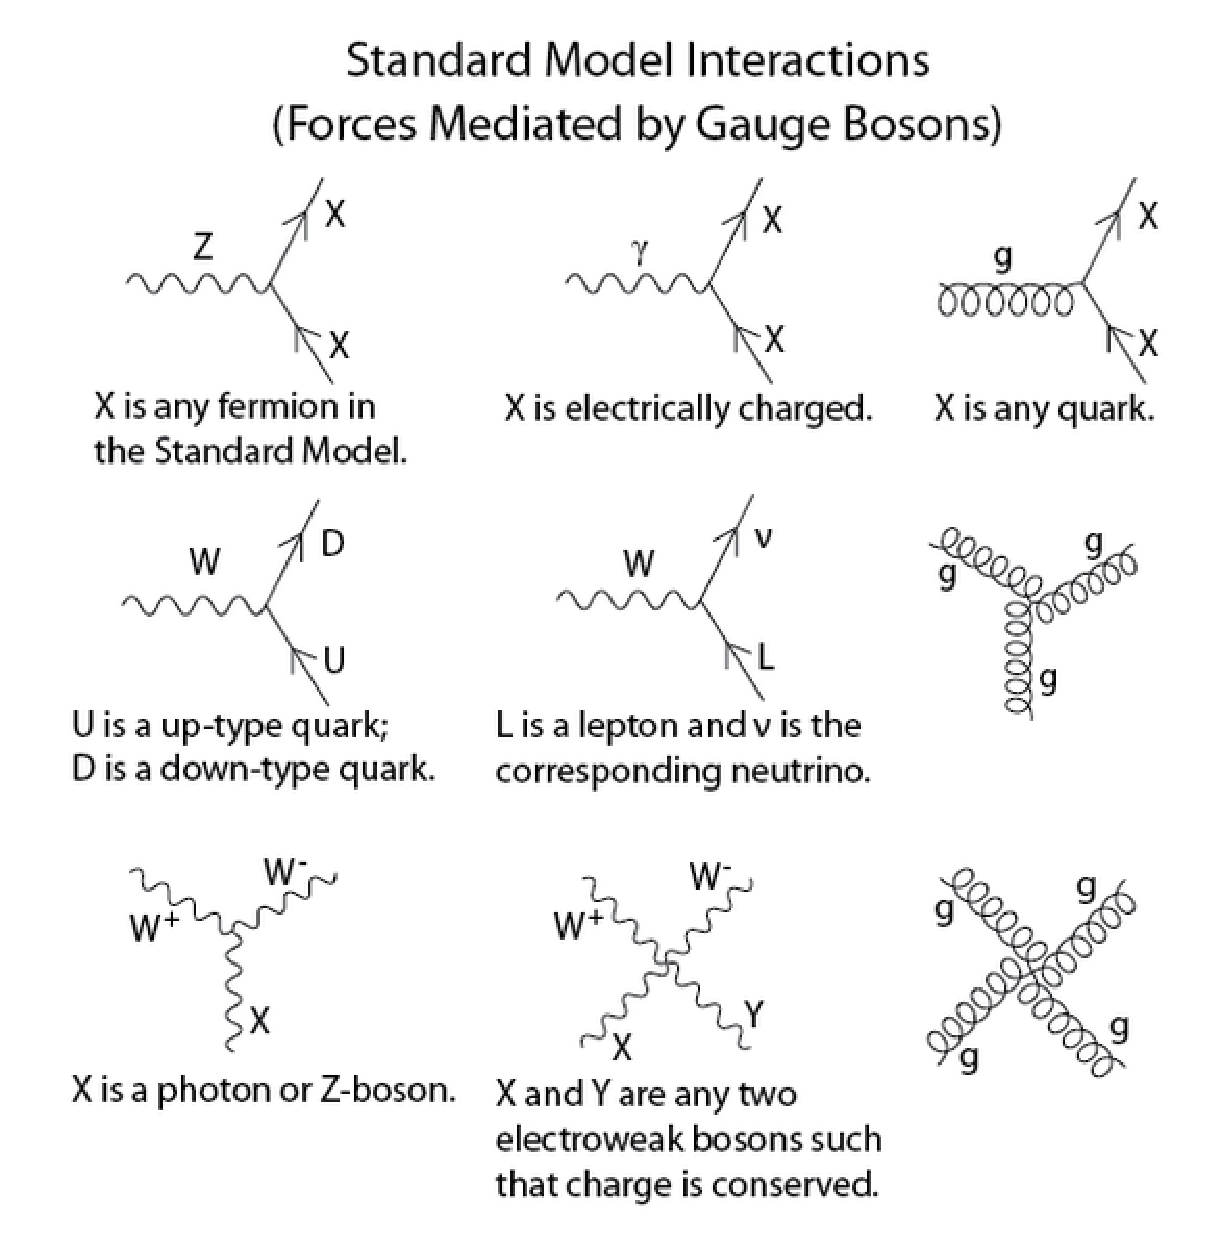
\includegraphics[width=0.70\textwidth]{figures/intro/Standard_Model_Feynman_Diagram_Vertices.pdf}
      \end{center}
\caption{Interactions of the SM in which the Higgs in not involved~\cite{SMinteractions_nonhiggs}.}
\label{fig:nonhiggsint}
\end{figure}

\section{Higgs Discovery\label{sec:discovery}}

While each particle has its own story of discovery, as hinted briefly by Figure~\ref{fig:discoveries},
this section will focus on that of the Higgs. What makes the search especially difficult is the
small couplings that the Higgs has with other particles, as shown in Figure~\ref{fig:crosssections}.
However, up until 2012, the mass of the Higgs boson was unknown, so big experimental searches
had to accommodate a wide range of possible values.

\begin{figure}[ht]
 \begin{center}
    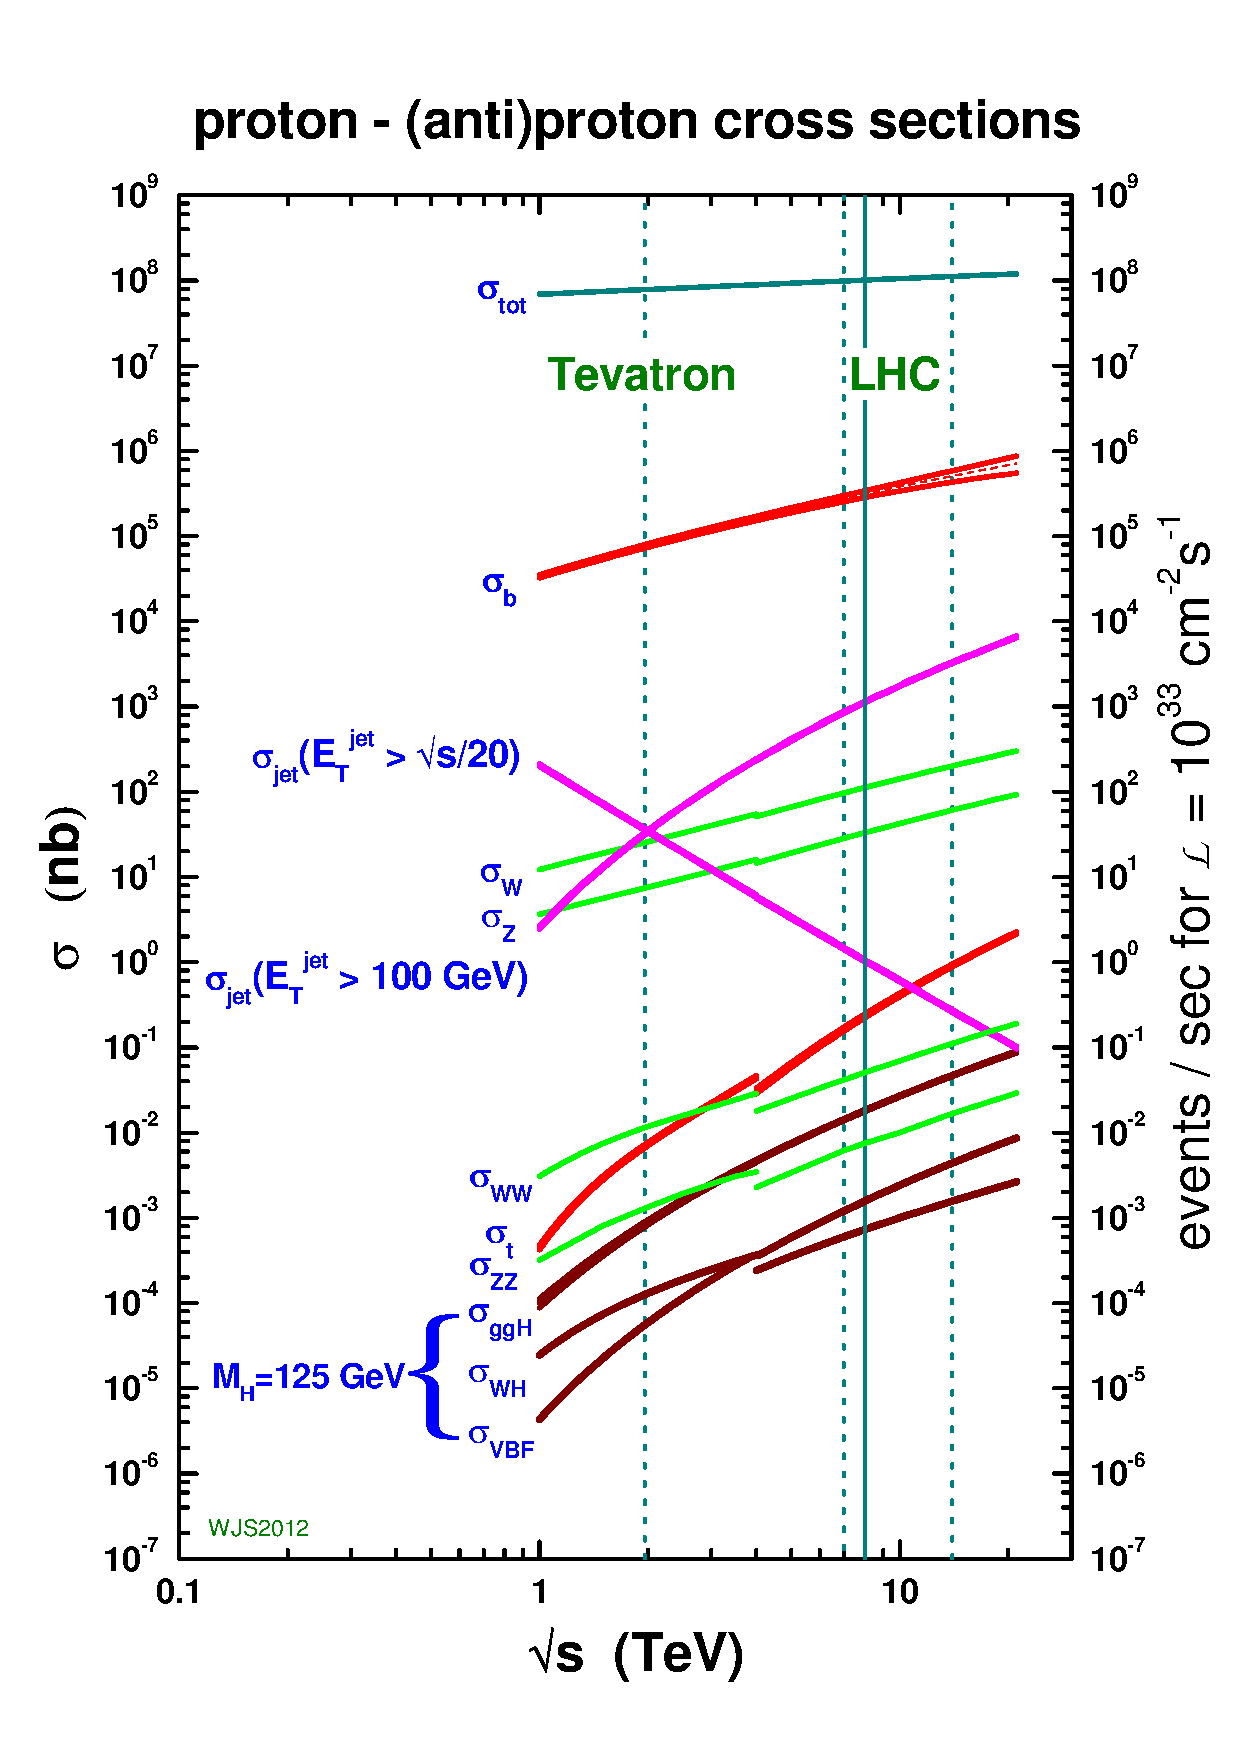
\includegraphics[width=0.80\textwidth]{figures/intro/crosssections2012_v5.pdf}
      \end{center}
\caption{Production cross sections for various processes in the SM versus center-of-mass energy.
The lower energies correspond to $p\bar{p}$ collisions from the Tevatron~\cite{Group:1984bk}, whereas
the higher energies correspond to $pp$ collisions from the LHC~\cite{cern-jinst-lhc}.}
\label{fig:crosssections}
\end{figure}

The search for the Higgs can be broken down into production mechanism and decay mode. For $pp$
collisions at $\sqrt{s} = 8$~TeV, as realized at the LHC, Figure~\ref{fig:higgsprod} shows the
dominant production mechanisms and corresponding cross sections. The branching ratios for several
decay modes are given in Table~\ref{table:BR_SMhiggs}. continue here!!!!!

\begin{figure}[ht]
 \begin{center}
    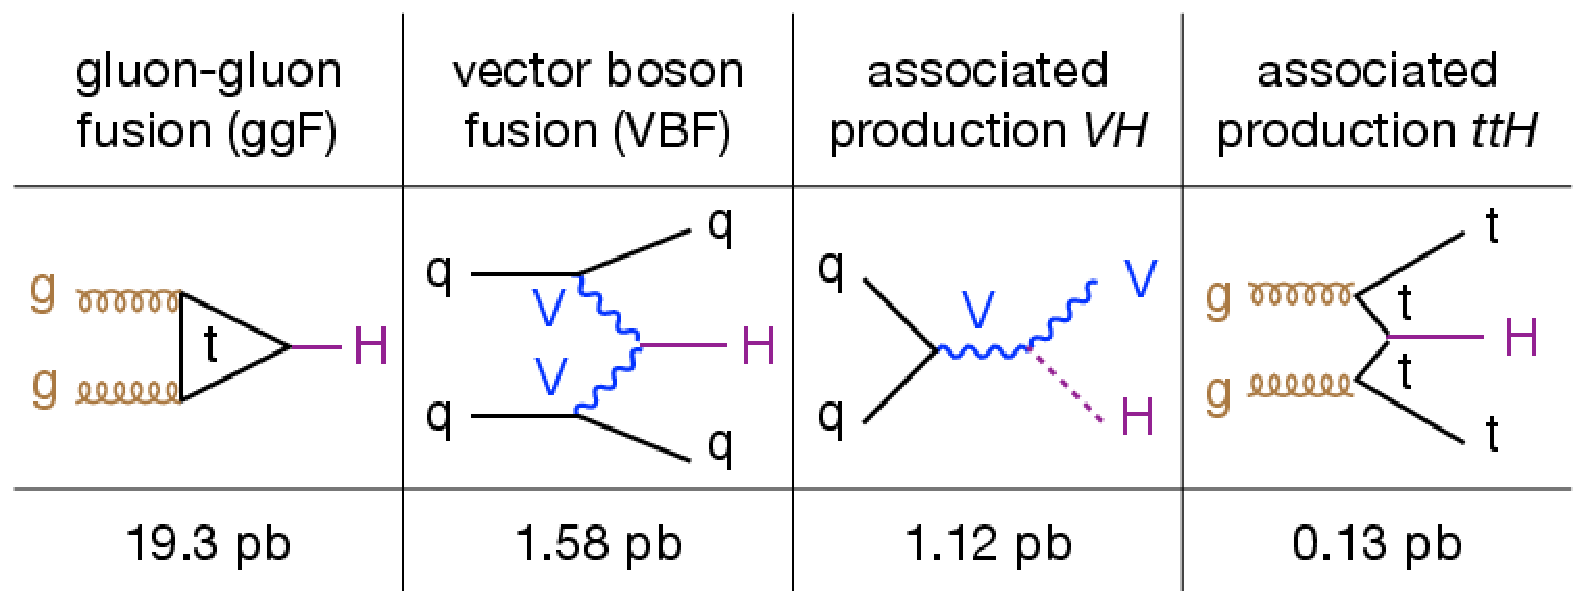
\includegraphics[width=0.90\textwidth]{figures/intro/higgsproductions.pdf}
      \end{center}
\caption{Production mechanisms and cross sections of the Higgs boson
for the leading processes in the SM~\cite{Tuna:thesis}. The cross sections correspond to
$pp$ collisions at $\sqrt{s} = 8$~TeV.}
\label{fig:crosssections}
\end{figure}

\begin{table}[bp]
  \centering
  \renewcommand{\arraystretch}{1.4}
  \caption{Branching ratios for the Higgs boson~\cite{LHC:SMHiggsBR}.}
  \begin{tabular}{|c|ccc|cccc|}
\hline
                     & \multicolumn{3}{c|}{fermions} & \multicolumn{4}{c}{bosons}  \\
  \hline
  Decay mode         & $bb$ & $\tau\tau$ & $\mu\mu$   & $WW^\ast$ & $ZZ^\ast$ & $\gamma\gamma$ & $Z\gamma$ \\
  Branching fraction & 58\% & 6.3\%     & 0.022\%    & 22\%      & 2.6\%     & 0.23\%         & 0.15\%    \\
\hline
\end{tabular}

  \label{table:BR_SMhiggs}
\end{table}


\section{Shortcomings of the SM\label{sec:SMshortcomings}}

There are both experimental and theoretical reasons for why the SM is not a complete theory of
particle physics. In some cases, the SM provides an ad-hoc description, and in other cases, there
is no description at all. For the optimist, these provide compelling reasons to continue
pushing the boundaries of our knowledge. Examples of such compelling questions concern gravity,
dark matter, dark energy, and neutrinos, as detailed in Subsections~\ref{subsec:grav},
\ref{subsec:dark}, and \ref{subsec:neu}, but this is not to omit other questions concerning,
for example, matter-antimatter asymmetry, hierarchy, dark energy, and generations of fermions.

\subsection{Gravity\label{subsec:grav}}

Gravity is well understood in the classical and relativistic limits, as first posited by Newton
and Einstein, respectively. However, there is no complete quantum theory of gravity, and as such
it is not accounted for by the SM. It is thought that the force is mediated by a spin-2 particle
called the gravition and that the gravitional force would unify with the other three forces
in a very-high energy limit.

\subsection{Dark Matter\label{subsec:dark}}

Ordinary matter, as built-up from the SM, only accounts for 15\% of the
matter in the universe~\cite{Clowe:2006eq}. The nature of the other 85\%, dubbed dark matter, is
largely unknown. Its presence is inferred from observing the way ordinary matter behaves at
astrophysical scales. In these observations, the behavior of certain objects cannot be explained
by the ordinary matter alone. Rather, it is posited that these observations can be explained by
the presence of some additional matter which interacts through gravity but not electromagnetism.
Candidate dark matter particles provide motivation for many experimental searches at the LHC and
other experiments.

\subsection{Neutrinos\label{subsec:neu}}

In the version of the SM presented in~\ref{sec:SM}, neutrinos are massless, electrically neutral
leptons which come in three flavors. The observation of neutrino oscillation~\cite{Fukuda:1998mi},
in which the probability of measuring a particular flavor in a neutrino varies over its trajectory,
implies that neutrinos have masses. These mass terms can and have been added to the SM, but it is
unclear if their origin is from the same mechanism that provides the other fermions with their
masses.

\section{diHiggs as a probe of SM and New Physics\label{sec:diHiggs}}


